\section{Line Integrals}\label{sec:line_int}

In single-variable calculus you learned how to integrate a real-valued function $f(x)$ over an interval $[a,b]$ in $\mathbb{R}^1$. This integral (usually called a \emph{Riemann integral})\index{Riemann integral} can be thought of as an integral over a \emph{path} in $\mathbb{R}^1$, since an interval (or collection of intervals) is really the only kind of ``path'' in $\mathbb{R}^1$. You may also recall that if $f(x)$ represented the force applied along the $x$-axis to an object at position $x$ in $[a,b]$, then the \emph{work} $W$ done in moving that object from position $x=a$ to $x=b$ was defined as the integral:
\[W=\int_a^b f(x)\,dx\]

In this section, we will see how to define the integral of a function (either real-valued or vector-valued) of two variables over a general path (i.e. a curve) in $\mathbb{R}^2$. This definition will be motivated by the physical notion of work. We will begin with real-valued functions of two variables.

In physics, the intuitive idea of work is that\index{work}
\[\text{Work} = \text{Force}\,\times\,\text{Distance} .\]
Suppose that we want to find the total amount $W$ of work done in moving an object along a curve $C$ in $\mathbb{R}^2$ with a smooth parametrization $x=x(t)$, $y=y(t)$, $a \le t \le b$, with a force $f(x,y)$ which varies with the position $(x,y)$ of the object and is applied in the direction of motion along $C$ (see \autoref{fig:lineintdef} below).

\begin{lxfigure}
 \begin{center}
  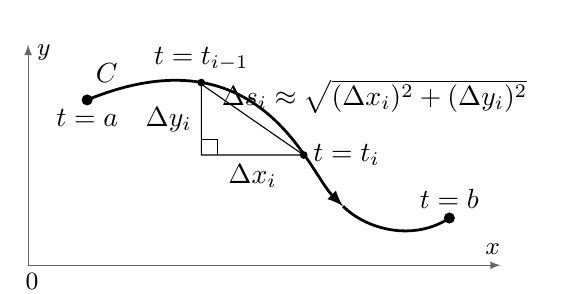
\begin{tikzpicture}
   \usetikzlibrary{arrows}
   \draw [black!60,line width=0.3pt,-latex] (0,0) -- (6,0,0);
   \draw [black!60,line width=0.3pt,-latex] (0,0) -- (0,2.8,0);
   \pgfputat{\pgfpointxyz{5.9}{0.2}{0}}{\pgfbox[center,center]{\small $x$}};
   \pgfputat{\pgfpointxyz{0.2}{2.7}{0}}{\pgfbox[center,center]{\small $y$}};
   \pgfputat{\pgfpointxyz{0.05}{-0.2}{0}}{\pgfbox[center,center]{\small $0$}};
   \draw [rounded corners,line width=1pt,-latex](0.75,2.1) .. controls (2.95,3) and (3.55,1.2) .. (4,0.75);
   \draw [rounded corners,line width=1pt] (4,0.75) .. controls (4.3,0.45) and (4.9,0.3) .. (5.35,0.6);
   \draw (2.2,2.3) -- (3.5,1.4) -- (2.2,1.4) -- (2.2,2.3);
   \draw (2.2,1.6) -- (2.4,1.6) -- (2.4,1.4);
   \node [left,above] at (1,2.2) {$C$};
   \fill (0.75,2.1) circle (2pt);
   \fill (5.35,0.6) circle (2pt);
   \fill (2.2,2.32) circle (1.4pt);
   \fill (3.5,1.4) circle (1.4pt);
   \node [below] at (0.75,2.1) {$t=a$};
   \node [above] at (5.35,0.6) {$t=b$};
   \node [right,above] at (4.4,1.8) {$\Delta s_i\approx\sqrt{(\Delta x_i)^2 + (\Delta y_i)^2}$};
   \node [above] at (2.2,2.35) {$t=t_{i-1}$};
   \node [right] at (3.5,1.4) {$t=t_i$};
   \node [left] at (2.2,1.85) {$\Delta y_i$};
   \node [below] at (2.85,1.4) {$\Delta x_i$};
  \end{tikzpicture}
 \end{center}
 \captionof{figure}{Curve $C:x=x(t),y=y(t)$ for $t$ in $[a,b]$}
 \label{fig:lineintdef}
\end{lxfigure}

We will assume for now that the function $f(x,y)$ is continuous and real-valued, so we only consider the magnitude of the force. Partition the interval $[a,b]$ as follows:
\[
 a = t_0 < t_1 < t_2 < \dots < t_{n-1} < t_n = b ,\text{ for some integer $n \ge 2$}
\]
As we can see from \autoref{fig:lineintdef}, over a typical subinterval $[t_{i-1},t_i]$ the distance $\Delta s_i$ traveled along the curve is approximately $\sqrt{(\Delta x_i)^2+(\Delta y_i)^2}$, by the Pythagorean Theorem. Thus, if the subinterval is small enough then the work done in moving the object along that piece of the curve is approximately
\[
 \text{Force}\,\times\,\text{Distance}
 \approx f(x_{i}^*,y_{i}^*)\,\sqrt{(\Delta x_i)^2 +(\Delta y_i)^2} ,
\]
where $(x_{i}^*,y_{i}^*)=(x(t_i^*),y(t_i^*))$ for some $t_i^*$ in $[t_{i-1},t_i]$, and so
\[
 W \approx \sum_{i=1}^n f(x_i^*,y_i^*)\,\sqrt{(\Delta x_i)^2 +(\Delta y_i)^2}
\]
is approximately the total amount of work done over the entire curve. But since
\[
 \sqrt{(\Delta x_i)^2+(\Delta y_i)^2}
 =\sqrt{\left(\frac{\Delta x_i}{\Delta t_i}\right)^2
 +\left(\frac{\Delta y_i}{\Delta t_i}\right)^2} \,\,\Delta t_i ,
\]
where $\Delta t_i=t_i-t_{i-1}$, then
\[
 W \approx \sum_{i=1}^n f(x_i^*,y_i^*)\,
 \sqrt{\left(\frac{\Delta x_i}{\Delta t_i}\right)^2
 +\left(\frac{\Delta y_i}{\Delta t_i}\right)^2} \,\Delta t_i .
\]
Taking the limit of that sum as the length of the largest subinterval goes to $0$, the sum over all subintervals becomes the integral from $t=a$ to $t=b$, $\frac{\Delta x_i}{\Delta t_i}$ and $\frac{\Delta y_i}{\Delta t_i}$ become $x\primeskip'(t)$ and $y\primeskip'(t)$, respectively, and $f(x_i^*,y_i^*)$ becomes $f(x(t),y(t))$, so that
\[
 W = \int_a^b f(x(t),y(t)) \,\sqrt{x\primeskip'(t)^2 + y\primeskip'(t)^2}\,dt .
\]

The integral on the right side of the above equation gives us our idea of how to define, for \emph{any} real-valued function $f(x,y)$, the integral of $f(x,y)$ along the curve $C$, called a \emph{line integral}:\index{line integral}\index{$\int_C$}

\definition{defn:lineintscalar2}{Line Integral of a Real Valued Function}{For a real-valued function $f(x,y)$ and a curve $C$ in $\mathbb{R}^2$, parametrized by $x=x(t)$, $y=y(t)$, $a \le t \le b$, the \textbf{line integral of} $f(x,y)$ \textbf{along} $C$ \textbf{with respect to arc length} $s$ is
 \[
  \int_C f(x,y)\,ds
  = \int_a^b f(x(t),y(t)) \,\sqrt{x\primeskip'(t)^2 + y\primeskip'(t)^2}\,\,dt .
 \]}

The symbol $ds$ is the differential of the arc length function
\[
 s = s(t) = \int_a^t \sqrt{x\primeskip'(u)^2 + y\primeskip'(u)^2}\,\,du ,
\]
which you may recognize from \autoref{sec:par_calc} as the length of the curve $C$ over the interval $[a,t]$, for all $t$ in $[a,b]$. That is,
\[
 ds = s\primeskip'(t)\,dt = \sqrt{x\primeskip'(t)^2 + y\primeskip'(t)^2}\,\,dt ,
\]
by the Fundamental Theorem of Calculus.

For a general real-valued function $f(x,y)$, what does the line integral $\int_C f(x,y)\,ds$ represent? The preceding discussion of $ds$ gives us a clue. You can think of differentials as infinitesimal lengths. So if you think of $f(x,y)$ as the height of a picket fence along $C$, then $f(x,y)\,ds$ can be thought of as approximately the area of a section of that fence over some infinitesimally small section of the curve, and thus the line integral $\int_C f(x,y)\,ds$ is the total area of that picket fence (see \autoref{fig:picketfence}).

\begin{lxfigure}
 \begin{center}
  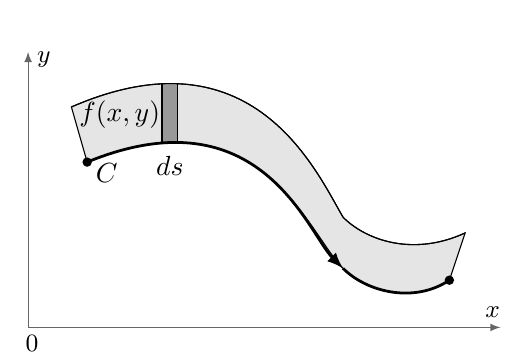
\begin{tikzpicture}
   \usetikzlibrary{arrows}
   \draw [black!60,line width=0.3pt,-latex] (0,0) -- (6,0,0);
   \draw [black!60,line width=0.3pt,-latex] (0,0) -- (0,3.5,0);
   \pgfputat{\pgfpointxyz{5.9}{0.2}{0}}{\pgfbox[center,center]{\small $x$}};
   \pgfputat{\pgfpointxyz{0.2}{3.4}{0}}{\pgfbox[center,center]{\small $y$}};
   \pgfputat{\pgfpointxyz{0.05}{-0.2}{0}}{\pgfbox[center,center]{\small $0$}};
   \filldraw [fill=black!10] (0.75,2.1) .. controls (2.95,3) and (3.55,1.2) .. (4,0.75) .. controls (4.3,0.45) and
    (4.9,0.3) .. (5.35,0.6) -- (5.55,1.2) .. controls (4.9,0.9) and (4.3,1.1) .. (4,1.4) .. controls (3.65,2) and
    (2.85,3.8) .. (0.55,2.8) -- (0.75,2.1);
   \fill [fill=black!40] (1.9,2.35) -- (1.9,3.1) -- (1.7,3.1) -- (1.7,2.35) -- (1.9,2.35);
   \draw (5.55,1.2) .. controls (4.9,0.9) and (4.3,1.1) .. (4,1.4) .. controls (3.65,2) and
    (2.85,3.8) .. (0.55,2.8);
   \draw [rounded corners,line width=1pt,-latex] (0.75,2.1) .. controls (2.95,3) and (3.55,1.2) .. (4,0.75);
   \draw [rounded corners,line width=1pt](4,0.75) .. controls (4.3,0.45) and (4.9,0.3) .. (5.35,0.6);
   \node [left,below] at (1,2.2) {$C$};
   \node [below] at (1.8,2.3) {$ds$};
   \draw (1.9,2.35) -- (1.9,3.1);
   \draw (1.7,2.35) -- (1.7,3.1);
   \node [left] at (1.8,2.7) {$f(x,y)$};
   \fill (0.75,2.1) circle (1.7pt);
   \fill (5.35,0.6) circle (1.7pt);
  \end{tikzpicture}\vspace{-5mm}
 \end{center}
 \captionof{figure}{Area of shaded rectangle $= \text{height}\times\text{width} \approx f(x,y)\,ds$}
 \label{fig:picketfence}
\end{lxfigure}

\example{exmp_lineintcyl}{Using the Line Integral}{Use a line integral to show that the lateral surface area $A$ of a right circular cylinder of radius $r$ and height $h$ is $2\pi r h$.}{%
 \mtable{Figure for \autoref{exmp_lineintcyl}}{fig_cyl_line_int}{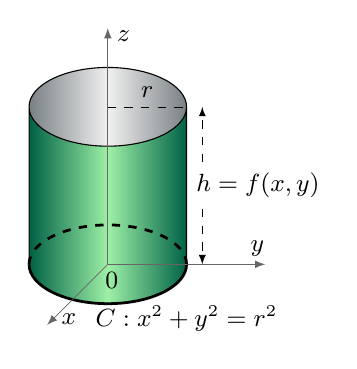
\begin{tikzpicture}
   \usetikzlibrary{arrows}
   \definecolor{insideo}{HTML}{798084}
   \definecolor{insidei}{HTML}{F0F0F0}
   \definecolor{outer}{HTML}{006146}
   \definecolor{inner}{HTML}{9EF0A6}
   \shade [left color=insideo,right color=insideo,middle color=insidei] (1,2) arc (0:180:1 and .5) --
    (-1,2) arc (180:360:1 and .5);
   \shadedraw [left color=outer,right color=outer,middle color=inner] (-1,0) arc (180:360:1 and .5) -- (1,2) --
    (1,2) arc (360:180:1 and .5) -- (-1,0);
   \draw (1,2) arc (0:180:1 and .5);
   \draw [line width=1pt] (-1,0) arc (180:360:1 and .5);
   \draw [dashed,line width=1pt] (1,0) arc (0:180:1 and .5);
   \draw [black!60,line width=0.3pt,-latex] (0,0) -- (2,0,0);
   \draw [black!60,line width=0.3pt,-latex] (0,0) -- (0,3,0);
   \draw [black!60,line width=0.3pt,-latex] (0,0) -- (0,0,2);
   \pgfputat{\pgfpointxyz{1.9}{0.2}{0}}{\pgfbox[center,center]{\small $y$}};
   \pgfputat{\pgfpointxyz{0.2}{2.9}{0}}{\pgfbox[center,center]{\small $z$}};
   \pgfputat{\pgfpointxyz{0.2}{0}{1.8}}{\pgfbox[center,center]{\small $x$}};
   \pgfputat{\pgfpointxyz{0.05}{-0.2}{0}}{\pgfbox[center,center]{\small $0$}};
   \draw [dashed,line width=0.2pt] (0,2) -- (1,2);
   \node [above] at (0.5,2) {\small $r$};
   \node [right] at (1,1) {\small $h=f(x,y)$};
   \draw [dashed,line width=0.2pt,-latex] (1.2,1.3) -- (1.2,2);
   \draw [dashed,line width=0.2pt,-latex] (1.2,0.7) -- (1.2,0);
   \node [right,below] at (1,-0.4) {\small $C: x^2 + y^2 = r^2$};
  \end{tikzpicture}}
We will use the right circular cylinder with base circle $C$ given by $x^2 + y^2 = r^2$ and with height $h$ in the positive $z$ direction (see \autoref{fig_cyl_line_int}). Parametrize $C$ as follows:
 \[
  x = x(t) = r \cos t ,\quad y = y(t) = r \sin t,\quad 0 \le t \le 2\pi
 \]
 Let $f(x,y) = h$ for all $(x,y)$. Then
 \begin{align*}
  A
  &= \int_C f(x,y)\,ds
   = \int_a^b f(x(t),y(t)) \,\sqrt{x\primeskip'(t)^2 + y\primeskip'(t)^2}\,\,dt\\
   &= \int_0^{2\pi} h \sqrt{(-r \sin t)^2 + (r \cos t)^2}\,\,dt\\
   &= h\int_0^{2\pi} r \sqrt{\sin^2 t + \cos^2 t}\,\,dt\\
   &= rh\int_0^{2\pi} 1 \,dt = 2\pi r h.\eoehere
 \end{align*}}

Note in \autoref{exmp_lineintcyl} that if we had traversed the circle $C$ twice, i.e. let $t$ vary from $0$ to $4\pi$, then we would have gotten an area of $4\pi r h$, i.e.\ twice the desired area, even though the \emph{curve} itself is still the same (namely, a circle of radius $r$). Also, notice that we traversed the circle in the counter-clockwise direction. If we had gone in the clockwise direction, using the parametrization
\begin{equation}\label{eqn:lineintcylcwise}
 x = x(t) = r \cos (2\pi - t) ,\quad y = y(t) = r \sin (2\pi - t),\quad 0 \le t \le 2\pi ,
\end{equation}
then it is easy to verify (see Exercise \ref{pr_double_circ}) that the value of the line integral is unchanged.

In general, it can be shown (see Exercise \ref{pr_rev_int}) that reversing the direction in which a curve $C$ is traversed leaves $\int_C f(x,y)\,ds$ unchanged, for any $f(x,y)$. If a curve $C$ has a parametrization $x=x(t)$, $y=y(t)$, $a \le t \le b$, then denote by $-C$ the same curve as $C$ but traversed in the opposite direction. Then $-C$ is parametrized by
\begin{equation}\label{eqn:reversec}
 x = x(a+b-t),\quad y = y(a+b-t),\quad a \le t \le b ,
\end{equation}
and we have
\[\int_C f(x,y)\,ds = \int_{-C} f(x,y)\,ds .\]

Notice that our definition of the line integral was with respect to the arc length parameter $s$. We can also define
\[
 \int_C f(x,y)\,dx = \int_a^b f(x(t),y(t)) \,x\primeskip'(t)\,dt
\]
as the \emph{line integral of $f(x,y)$ along $C$ with respect to $x$}, and
\[
 \int_C f(x,y)\,dy = \int_a^b f(x(t),y(t)) \,y\primeskip'(t)\,dt
\]
as the \emph{line integral of $f(x,y)$ along $C$ with respect to $y$}.

In the derivation of the formula for a line integral, we used the idea of work as force multiplied by distance. However, we know that force is actually a \emph{vector}. So it would be helpful to develop a vector form for a line integral. For this, suppose that we have a function $\textbf{f}(x,y)$ defined on $\mathbb{R}^2$ by
\[\textbf{f}(x,y) = P(x,y)\,\textbf{i} + Q(x,y)\,\textbf{j}\]
for some continuous real-valued functions $P(x,y)$ and $Q(x,y)$ on $\mathbb{R}^2$. Such a function \textbf{f} is called a \textbf{vector field} on $\mathbb{R}^2$. It is defined at \emph{points} in $\mathbb{R}^2$, and its values are \emph{vectors} in $\mathbb{R}^2$. For a curve $C$ with a smooth parametrization $x=x(t)$, $y=y(t)$, $a \le t \le b$, let\index{vector field}
\[\textbf{r}(t) = x(t)\,\textbf{i} + y(t)\,\textbf{j}\]
be the position vector for a point $(x(t),y(t))$ on $C$. Then\index{position vector} $\textbf{r}\primeskip'(t) = x\primeskip'(t)\,\textbf{i} + y\primeskip'(t)\,\textbf{j}$ and so
\begin{align*}
 \int_C P(x,y)\,dx + \int_C Q(x,y)\,dy
 &= \int_a^b P(x(t),y(t)) \,x\primeskip'(t)\,dt + \int_a^b Q(x(t),y(t)) \,y\primeskip'(t)\,dt\\
  &= \int_a^b (P(x(t),y(t)) \,x\primeskip'(t) + Q(x(t),y(t)) \,y\primeskip'(t))\,dt\\
  &= \int_a^b \dotp{f(x(t),y(t))}{r\primeskip'(t)}\,dt
\end{align*}
by definition of $\textbf{f}(x,y)$. Notice that the function $\dotp{f(x(t),y(t))}{r\primeskip'(t)}$ is a \emph{real-valued} function on $[a,b]$, so the last integral on the right looks somewhat similar to our earlier definition of a line integral. This leads us to the following definition:\index{line integral}\index{$\int_C$}

\definition{defn:lineintvec2}{Line Integral of a Vector Valued Function}{For a vector field $\textbf{f}(x,y) = P(x,y)\,\textbf{i} + Q(x,y)\,\textbf{j}$ and a curve $C$ with a smooth parametrization $x=x(t)$, $y=y(t)$, $a \le t \le b$, the \textbf{line integral of f along} $C$ is
 \begin{align}
  \int_C \dotp{f}{dr}
  &= \int_C P(x,y)\,dx + \int_C Q(x,y)\,dy\\
   &= \int_a^b \dotp{f(x(t),y(t))}{r\primeskip'(t)}\,dt ,
 \end{align}
 where $\textbf{r}(t) = x(t)\,\textbf{i} + y(t)\,\textbf{j}$ is the position vector for points on $C$.}

We use the notation $d\textbf{r} = \textbf{r}\primeskip'(t)\,dt = dx\,\textbf{i} + dy\,\textbf{j}$\index{$d\textbf{r}$} to denote the \textbf{differential}\index{differential} of the vector-valued function \textbf{r}. The line integral in \autoref{defn:lineintvec2} is often called a \emph{line integral of a vector field} to distinguish it from the line integral in \autoref{defn:lineintscalar2} which is called a \emph{line integral of a scalar field}. For convenience we will often write
\[\int_C P(x,y)\,dx + \int_C Q(x,y)\,dy = \int_C P(x,y)\,dx + Q(x,y)\,dy ,\]
where it is understood that the line integral along $C$ is being applied to both $P$ and $Q$. The quantity $P(x,y)\,dx + Q(x,y)\,dy$ is known as a \textbf{differential form}.\index{differential form} For a real-valued function $F(x,y)$, the \textbf{differential} of $F$ is $dF = \frac{\partial F}{\partial x}\,dx + \frac{\partial F}{\partial y}\,dy$. A differential form $P(x,y)\,dx + Q(x,y)\,dy$ is called \textbf{exact}\index{exact differential form} if it equals $dF$ for some function $F(x,y)$.

Recall that if the points on a curve $C$ have position vector $\textbf{r}(t) = x(t)\,\textbf{i} + y(t)\,\textbf{j}$, then $\textbf{r}\primeskip'(t)$ is a tangent vector to $C$ at the point $(x(t),y(t))$ in the direction of increasing $t$ (which we call the \emph{direction of $C$}). Since $C$ is a smooth curve, then $\textbf{r}\primeskip'(t) \ne \textbf{0}$ on $[a,b]$ and hence
\[\textbf{T}(t) = \frac{\textbf{r}\primeskip'(t)}{\norm{\textbf{r}\primeskip'(t)}}\]
is the unit tangent vector to $C$ at $(x(t),y(t))$. Putting Definitions \ref{defn:lineintscalar2} and \ref{defn:lineintvec2} together we get the following theorem:

\theorem{thm:lineinttangent}{Line Integrals and Tangent Vectors}{For a vector field $\textbf{f}(x,y) = P(x,y)\,\textbf{i} + Q(x,y)\,\textbf{j}$ and a curve $C$ with a smooth parametrization $x=x(t)$, $y=y(t)$, $a \le t \le b$ and position vector $\textbf{r}(t) = x(t)\,\textbf{i} + y(t)\,\textbf{j}$,
 \[
  \int_C \dotp{f}{dr}
  = \int_C \dotp{f}{T}\,ds ,
 \]
 where $\textbf{T}(t) = \frac{\textbf{r}\primeskip'(t)}{\norm{\textbf{r}\primeskip'(t)}}$ is the unit tangent vector to $C$ at  $(x(t),y(t))$.}

If the vector field $\textbf{f}(x,y)$ represents the force moving an object along a curve $C$, then the work $W$ done by this force is
\[
 W = \int_C \dotp{f}{T}\,ds
 = \int_C \dotp{f}{dr} .
\]

\example{exmp_lineintexmp}{Evaluating Line Integrals}{Evaluate $\int_C (x^2 + y^2 )\,dx + 2xy\,dy$, where:
 \begin{enumerate}
  \item $C: x=t,\quad y=2t,\quad 0 \le t \le 1$
  \item $C: x=t,\quad y=2t^2 ,\quad 0 \le t \le 1$
 \end{enumerate}}{%
%
 \mtable{Figure for \autoref{exmp_lineintexmp}}{fig_line_ints}{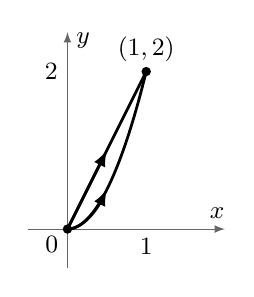
\begin{tikzpicture}
   \usetikzlibrary{arrows}
   \draw [black!60,line width=0.3pt,-latex] (-0.5,0) -- (2,0);
   \draw [black!60,line width=0.3pt,-latex] (0,-0.5) -- (0,2.5);
   \pgfputat{\pgfpointxyz{1.9}{0.2}{0}}{\pgfbox[center,center]{\small $x$}}
   \pgfputat{\pgfpointxyz{0.2}{2.4}{0}}{\pgfbox[center,center]{\small $y$}}
   \pgfputat{\pgfpointxyz{-0.2}{-0.2}{0}}{\pgfbox[center,center]{\small $0$}}
   \draw [line width=1pt] (0,0) parabola (1,2);
   \draw [line width=1pt,-latex] (0,0) parabola (0.5,0.5);
   \draw [line width=1pt] (0,0) -- (1,2);
   \draw [line width=1pt,-latex] (0,0) -- (0.5,1);
   \node [right,above] at (1,2) {\small $(1,2)$};
   \node [left] at (0,2) {\small $2$};
   \node [below] at (1,0) {\small $1$};
   \fill (0,0) circle (1.7pt);
   \fill (1,2) circle (1.7pt);
  \end{tikzpicture}}
  %
 \autoref{fig_line_ints} shows both curves.
 \begin{enumerate}
 \item Since $x\primeskip'(t)=1$ and $y\primeskip'(t)=2$, then
 \begin{align*}
  \int_C (x^2 + y^2 )\,dx + 2xy\,dy &=
   \int_0^1 \left( ( x(t)^2 + y(t)^2 )x\primeskip'(t) + 2x(t)y(t)\,y\primeskip'(t) \right) \,dt\\
   &= \int_0^1 \left( (t^2 + 4t^2 )(1) + 2t(2t)(2) \right) \,dt\\
   &= \int_0^1 13t^2 \,dt\\
   &= \frac{13t^3}{3}\,\Bigg|_0^1 = \frac{13}{3}
 \end{align*}

 \item Since $x\primeskip'(t)=1$ and $y\primeskip'(t)=4t$, then
 \begin{align*}
  \int_C (x^2 + y^2 )\,dx + 2xy\,dy &=
   \int_0^1 \left( ( x(t)^2 + y(t)^2 )x\primeskip'(t) + 2x(t)y(t)\,y\primeskip'(t) \right) \,dt\\
   &= \int_0^1 \left( (t^2 + 4t^4 )(1) + 2t(2t^2 )(4t) \right) \,dt\\
   &= \int_0^1 (t^2 + 20t^4 )\,dt\\
   &= \frac{t^3}{3} + 4t^5 \,\Bigg|_0^1 = \frac{1}{3} + 4 = \frac{13}{3}
 \end{align*}
 So in both cases, if the vector field $\textbf{f}(x,y) = ( x^2 + y^2 )\,\textbf{i} + 2xy\,\textbf{j}$ represents the force moving an object from $(0,0)$ to $(1,2)$ along the given curve $C$, then the work done is $\frac{13}{3}$. This may lead you to think that work (and more generally, the line integral of a vector field) is independent of the path taken. However, as we will see in the next section, this is not always the case.\eoehere
 \end{enumerate}}

Although we defined line integrals over a single smooth curve, if $C$ is a \emph{piecewise smooth curve}, that is\index{piecewise smooth curve}
\[C = C_1 \cup C_2 \cup \ldots \cup C_n\]
is the union of smooth curves $C_1,\dotsc,C_n$, then we can define
\[
 \int_C \dotp{f}{dr}
  = \int_{C_1} \dotp{f}{dr_1} +
  \int_{C_2} \dotp{f}{dr_2} + \dotsb +
  \int_{C_n} \dotp{f}{dr_n}
\]
where each $\textbf{r}_i$ is the position vector of the curve $C_i$.

\example{exmp_lineintexmppoly}{A Piecewise Smooth Line Integral}{Evaluate $\int_C (x^2 + y^2 )\,dx + 2xy\,dy$, where $C$ is the polygonal path from $(0,0)$ to $(0,2)$ to $(1,2)$.}{%
%
 \mtable{The Figure for \autoref{exmp_lineintexmppoly}}{fig_piece_line_int}{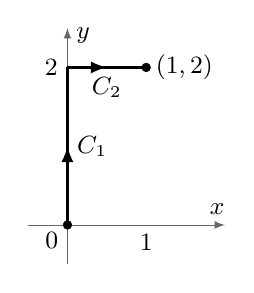
\begin{tikzpicture}
   \usetikzlibrary{arrows}
   \draw [black!60,line width=0.3pt,-latex] (-0.5,0) -- (2,0);
   \draw [black!60,line width=0.3pt,-latex] (0,-0.5) -- (0,2.5);
   \pgfputat{\pgfpointxyz{1.9}{0.2}{0}}{\pgfbox[center,center]{\small $x$}}
   \pgfputat{\pgfpointxyz{0.2}{2.4}{0}}{\pgfbox[center,center]{\small $y$}}
   \pgfputat{\pgfpointxyz{-0.2}{-0.2}{0}}{\pgfbox[center,center]{\small $0$}}
   \draw [line width=1pt] (0,0) -- (0,2);
   \draw [line width=1pt,-latex] (0,0) -- (0,1);
   \draw [line width=1pt] (0,2) -- (1,2);
   \draw [line width=1pt,-latex] (0,2) -- (0.5,2);
   \node [right] at (1,2) {\small $(1,2)$};
   \node [left] at (0,2) {\small $2$};
   \node [below] at (1,0) {\small $1$};
   \node [right] at (0,1) {\small $C_1$};
   \node [below] at (0.5,2) {\small $C_2$};
   \fill (0,0) circle (1.7pt);
   \fill (1,2) circle (1.7pt);
  \end{tikzpicture}}
  %
Write $C=C_1\cup C_2$, where $C_1$ is the curve given by $x=0$, $y=t$, $0 \le t \le 2$ and $C_2$ is the curve given by $x=t$, $y=2$, $0 \le t \le 1$ (see \autoref{fig_piece_line_int}). Then
 \begin{align*}
  \int_C (x^2 + y^2 )\,dx + 2xy\,dy
  &= \int_{C_1} (x^2 + y^2 )\,dx + 2xy\,dy\\
   &+ \int_{C_2} (x^2 + y^2 )\,dx + 2xy\,dy\\[6pt]
   &= \int_0^2 \left( (0^2 + t^2 )(0) + 2(0)t(1) \right) \,dt +
    \int_0^1 \left( (t^2 + 4 )(1) + 2t(2)(0) \right) \,dt\\[6pt]
   &= \int_0^2 0\,dt + \int_0^1 (t^2 + 4 )\,dt\\[6pt]
   &= \frac{t^3}{3} + 4t \,\Bigg|_0^1 = \frac{1}{3} + 4 = \frac{13}{3}\eoehere
 \end{align*}}

Line integral notation varies quite a bit. For example, in physics it is common to see the notation $\int_a^b \dotp{f}{dl}$, where it is understood that the limits of integration $a$ and $b$ are for the underlying parameter $t$ of the curve, and the letter \textbf{l} signifies length. Also, the formulation $\int_C \dotp{f}{T}\,ds$ from \autoref{thm:lineinttangent} is often preferred in physics since it emphasizes the idea of integrating the tangential component $\dotp{f}{T}$ of \textbf{f} in the direction of \textbf{T} (i.e. in the direction of $C$), which is a useful physical interpretation of line integrals.

\printexercises{exercises/14_Line_Int_exercises}
